%=====================================================================================================

%       Math 244 Lecture Notes

%       Chapters 22 Day Three (Means)

%				201701

%				LaTeX=>PDF sizing, graphics
%=====================================================================================================


\documentclass[12pt]{amsart}
\usepackage{amssymb,latexsym}
\usepackage{graphicx}
\usepackage{multicol}
\usepackage{multirow}
\usepackage{amsmath}
\usepackage{calc}
\usepackage{enumitem}
\usepackage{fancyhdr,lastpage}
\usepackage{setspace}
\usepackage{caption}
\usepackage{framed}
\usepackage{wasysym}

\theoremstyle{definition}
\pagestyle{fancy}
\newtheorem{theorem}{Theorem}
\newtheorem{lemma}{Lemma}
\newtheorem{defi}{Definition}
\newtheorem*{notation}{Notation}
\newtheorem{ex}{Example}
\newtheorem{proc}{Process}
\newtheorem{gw}{Group Work}
\newtheorem*{summary}{}

\setlength{\textwidth}{7.25in}			%for =>PDF, use 6.5in
\setlength{\textheight}{9.5in}		%for =>PDF, use 9.5in
\setlength{\oddsidemargin}{-0.375in}		
\setlength{\evensidemargin}{-0.375in}		
\setlength{\voffset}{-.75in}			%for=>PDF, use -0.75in
\setlength{\footskip}{15pt}


% For degree symbol
\newcommand{\degree}{\ensuremath{^\circ}}



% enumerate settings
\setlist{itemsep=4pt}	%topsep=0.1em
\renewcommand{\labelenumi}{ (\alph{enumi}) }			% makes enumeration (a) instead of (a).



\usepackage{placeins} % enables \FloatBarrier, useful for positioning figures/tables more precisely.
%\usepackage[dvips]{graphics}
%\usetikzlibrary{arrows}


\usepackage{pgfplots}

\tikzset{>=stealth}
\usetikzlibrary{backgrounds,arrows}
\tikzset{tight background}


\pgfplotsset{every axis/.append style={width=6.75cm,height=6.75cm,
					axis x line=middle,
					axis y line=middle,
					line width=0.75pt,
					tick label style={font=\tiny},
					label style={font=\small},
					legend style={font=\tiny}
}}

\pgfplotsset{framed/.style={axis background/.style ={draw=black!75}}}

\pgfmathdeclarefunction{gauss}{3}{%
	\pgfmathparse{1/(#3*sqrt(2*pi))*exp(-((#1-#2)^2)/(2*#3^2))}%
}



\usepackage{hyperref}
%\usepackage{url}
\hypersetup{colorlinks=true,urlcolor=blue,linkcolor=blue,breaklinks=true}

\usepackage{xcolor}
%		My colors
\definecolor{silver}{rgb}{0.95,0.95,0.95}
\definecolor{mypurple}{cmyk}{0.5,1,0,0}			%purple
\definecolor{myblue}{cmyk}{1,0.012,0,0}		%blue
\definecolor{mygreen}{cmyk}{1,0,0.99995,0}		%green
\definecolor{myred}{cmyk}{0,1,1,0}


\setlength{\parindent}{0pt}

\date{}



\begin{document}

\newcommand{\ph}{\phantom}
\newcommand{\ds}{\displaystyle}

\renewcommand{\emph}{\textbf}
\onehalfspace

%============================================================
%           Header Stuff   CHANGE FOR EACH SECTION!!!
%============================================================

\fancyhf{}   % clears both header and footer
\fancyfoot[RE,RO]{ \scriptsize{Page \thepage\ of \pageref{LastPage}}}
\fancyfoot[LE,LO]{\scriptsize{Instructor:  J.Wherry}}
\fancyhead[RE,RO]{\scriptsize{Chapter 22 Revisited: Comparing Two independent Means }}
\fancyhead[LE,LO]{\scriptsize{Math 244 Lecture Notes }}
\renewcommand{\headrulewidth}{0.4pt} % Removes header line if 0pt
\fancyfootoffset[LE,LO]{0in}        %Moves center ??
\renewcommand{\footrulewidth}{0.4pt} % Removes header line if 0pt



%============================================================
%           Title/ Info
%============================================================

\begin{center}

	\larger[3]	Math 244 Lecture Notes \smaller[3]		\\[22pt]

\end{center}

\section*{Chapter 22 Revisited: Comparing Two independent Means}




 \textbf{Overview:} Today, we will compare the sample averages for two groups using both confidence intervals and hypothesis tests. This will use many of the techniques from the previous chapters.
 ~\\
 
 \begin{framed}
  We found our confidence interval for one-sample average using the formula $$\bar{x}\pm t_{df}^* \frac{s}{\sqrt{n}}$$ or rather (Center)$\pm$(Dist$)^*$SE. Confidence intervals are based off \underline{\hspace{1in}}
 \end{framed}
 
\begin{framed}
We used the model in step two of a hypothesis test of $$\bar{X}\approx t_{df}\left(\mu, \frac{s}{\sqrt{n}}\right)$$ Hypothesis tests are based off \underline{\hspace{1in}}.
\end{framed}

Both our CI and our H-Test were created from the same model. So, if we have a model for comparing two independent averages, we'll be able to test claims and determine the actual difference in two groups.\\
~\\
\begin{ex} Suppose that $\mu_{Safeway}-\mu_{Grocery Outlet}>0$ for the average cost for a weeks worth of groceries at the two stores. Which store costs more?\end{ex} \vfill

\begin{ex} Suppose that $\mu_{Safeway}-\mu_{Fred Meyer}<0$ for the average cost for a weeks worth of groceries at the two stores. Which store costs more?\end{ex} \vfill

\begin{ex} Suppose that $\mu_{Safeway}-\mu_{Albertsons}=0$ for the average cost for a weeks worth of groceries at the two stores. Which store costs more?\end{ex} \vfill

NOTE:
\newpage
We need a model for $\bar{X}_2-\bar{X}_1$. We start with some quick observations...
\begin{enumerate}
 \item The model for a single average, CLT, is $$\bar{X}_1\approx t_{df}\left(\mu_1, \frac{s_1}{\sqrt{n_1}}\right)=t_{df}\left(\mu_1, \sqrt{\frac{s_1^2}{n_1}}\right).$$
 \item Much like the normal distribution: If you add/subtract two t-distribution models, you will get another t-distribution model.
 \item If $X$ and $Y$ are independent variables, then $$Var[X-Y]=Var[X]+Var[Y].$$
\end{enumerate}

Our model for $\bar{X}_2-\bar{X}_1$ is still a t-distribution based off the second fact. Let's determine which t-distribution.

\begin{ex} CENTER: $E[\bar{X}_1]=\mu_1$ and $E[\bar{X}_2]=\mu_2$ are the centers for each of our individual models. What is the center for $E[\bar{X}_1-\bar{X}_2]$?
\end{ex}

\vspace{1in}

\begin{ex} VARIANCE: $Var[\bar{X}_1]=\frac{s_1^2}{n_1}$ and $Var[\bar{X}_2]=\frac{s_2^2}{n_2}$ are the variances for each of our individual models. What is the variance for the difference, $Var[\bar{X}_1-\bar{X}_2]$?
\end{ex}

\vspace{1.5in}

\begin{ex}Based off the variance, what is the standard deviation, $SD[\bar{X}_1-\bar{X}_2]$?
\end{ex}
\vspace{0.5in}
\begin{framed}
 Our model is
 
 \vspace{0.75in}
 
\end{framed}
\newpage
NOTE: The actual df is $\displaystyle df=\frac{\left(\frac{s_1^2}{n_1}+\frac{s_2^2}{n_2}\right)^2}{\frac{1}{n_1-1}\left(\frac{s_1^2}{n_1}\right)^2+\frac{1}{n_2-1}\left(\frac{s_2^2}{n_2}\right)^2}$. This is often not a whole number.\\
~\\
\begin{framed}
 Mr. Wherry's Lie: Let $df=\min{df_1,df_2}$. Our intervals and H-tests should be close to the actual results even though our df will appear very different. 
\end{framed}

\begin{ex} 
 Find df for comparing two independent means if $n_1=100$ and $n_2=31$.
\end{ex}

\begin{ex}
 Find df for comparing two independent means if $n_1=11$ and $n_2=200$.
\end{ex}

\vspace{0.1in}

\hrule

\vspace{0.1in}

\begin{ex}
Using the model $$\bar{X}_1-\bar{X}_2\approx t_{df}\left( \mu_1-\mu_2, \sqrt{\frac{s_1^2}{n_1}+\frac{s_2^2}{n_2}}\right)$$ create the confidence interval for $\mu_1-\mu_2$.\\
HINT: Our interval will be based off samples and look something like (Center)$\pm t^*$ SE.
\end{ex}

\vspace{0.5in}

Our assumptions are...
\begin{enumerate}
 \item \,
 \item \,
 \item \, 
 \item \,
\end{enumerate}

\begin{ex} Create a $90\%$ CI for $\mu_1-\mu_2$ if $\bar{x_1}=3\,hrs$, $s_1=2\,hrs$, $n_1=25$, $\bar{x_2}=8\,hrs$, $s_2=1\,hr$, and $n_2=50$.
\end{ex}

\vspace{2in}

Which group appears to have a larger average? Why?

\vspace{.25in}

\newpage
 \begin{ex} Suppose you got a $95\%$ CI for the average jumping difference in feet, $\mu_{Victor}-\mu_{Fiona}$, of $(-0.04,-0.03)$. What does this tell us?
 \end{ex}
 
 \vfill
 
\begin{ex} Suppose you got a $95\%$ CI for the average jumping difference in feet, $\mu_{Victor}-\mu_{Fiona}$, of $(-0.04,0.10)$. What does this tell us?
 \end{ex}
 
 \vfill
 
 \begin{ex} Suppose you got a $95\%$ CI for the average jumping difference in feet, $\mu_{Victor}-\mu_{Fiona}$, of $(-0.04,-0.03)$.  What would the $95\%$ for $\mu_{Fiona}-\mu_{Victor}$ look like?\end{ex}
 
 \vfill

 
 \begin{ex} During a clinical study it is found that Tylenol lasts $4$ hours for headache relief on average with a standard deviation of $0.5$ hrs in $150$ trials. In contrast, Advil lasts $6$ hours for headache relief on average with a standard deviation of $3$ hrs in $100$ trials. Compare the groups using a $90\%$ CI. Check the assumptions assuming that patients were selected at random from hospitals throughout the nation. \end{ex}
 \vfill
 \vfill
 \newpage
\begin{ex} Recall that during a clinical study it is found that Tylenol lasts $4$ hours for headache relief on average with a standard deviation of $0.5$ hrs in $150$ trials. In contrast, Advil lasts $6$ hours for headache relief on average with a standard deviation of $3$ hrs in $100$ trials. This time, however, let's use a hypothesis test to test if ``Advil lasts longer the Tylenol``.\end{ex}

STEP I:

\vspace{0.5in}

STEP II: We already have the model: $\bar{X}_1-\bar{X}_2\approx t_{df}\left( \mu_1-\mu_2, \sqrt{\frac{s_1^2}{n_1}+\frac{s_2^2}{n_2}}\right)$. So, let's check assumptions and fill in numbers.

\vspace{1in}

STEP III:

\vfill

Step IV: What $\alpha$ should we use to be consistent?
\vspace{0.5in}

\newpage
\noindent \textbf{Checking CI with Calculator:} In our calculator, we use ``2-sampletInt" to check our interval. This is found in either [Stat]$\rightarrow$[Tests] on the TI-83/84 OR [Stat/List]$\rightarrow$[F7:Ints] on the TI-89. Type in your relevant information and you are good to go!\\
~\\
Calc Interval:\\
~\\
\noindent \textbf{Checking H-Test with Calculator:} In our calculator, we use ``2-sampletTest" to check our hypothesis test. This is found in either [Stat]$\rightarrow$[Tests] on the TI-83/84 OR [Stat/List]$\rightarrow$[F6:Tests] on the TI-89. Type in your relevant information and you are good to go!\\
~\\
Calc P-Value:\\
~\\
\hrule
~\\
\begin{ex}
 Sonya is preparing her spring garden. Last year, she bought sunflower starters from Al's Garden Store and Orchard's Supply Store. Sonya believes that the sunflowers from Al's are taller on average. After collecting some data, she found that for the $50$ sunflowers bought at Al's, plants grew to be an average of $6.3$ feet with a standard deviation of $1.2$ feet. In contrast, the $25$ sunflowers she bought from Orchard's, which ended up having a unimodal/symmetric height histogram, grew to $4.8$ feet on average with a standard deviation of $2$ feet. Test for a difference in heights and follow it up with the appropriate level confidence interval. Be sure to check assumptions.
\end{ex}
\vfill
\newpage
\begin{ex}
	A survey done at the Oregon Zoo finds that out of $200$ people sampled (various days and times) people spent $\$10.72$ per person on average with a standard deviation of $\$1.35$. In contrast, people at OMSI spent $\$13$ per person with a standard deviation of $\$5$ in a survey of $150$ people. Test if OMSI costs more on average than the Oregon Zoo.
\end{ex}

\begin{ex}
	The owners of Cinetopia sample $100$ movies from the last $4$ years and find that they have an average run length of $100\,mins$ with a standard deviation of $18\,mins$. The local Regal does a similar survey and finds an average of $120\,mins$ with a standard deviation of $30\,mins$ for $80$ samples. Test if there is a difference in average run length between the theaters.
\end{ex}

\begin{ex}
	Barry Allen is training for the mile. In a recent study at STAR Labs, it was determined that he's running an average mile time of $0.1$ second with a standard deviation of $0.01$ seconds for a collection of $52$ samples. Wally West thinks he is faster. He can run the mile in $0.099$ seconds with a standard deviation of $0.1$ second for a collection of $1000$ samples. Test if Wally is faster.
\end{ex}

\begin{ex}
	Claire works as a night nurse. She samples $50$ individuals and finds that they have an average hospital bill of $\$3,200$ for one night with a standard deviation of $\$700$. Blue Cross/Blue Shield reports a cost of $\$4,000$ on average with a standard deviation of $\$1000$ for a sample of $200$. Test if Claire's local hospital is cheaper on average. 
\end{ex}

\begin{ex}
	Mr. Wherry is training his cat, Fiona, for the Cat Olympics. She is known for her high jump. Curious as to what her true average high jump height is, Mr. Wherry measures several jump heights and gets the following data in feet: $4.5$, $4.75$, $4.75$, $4.8$, $4.8$, $4.8$, $4.8$, $5$, $5$, and $5.25$. Victor, Mr. Wherry's other cat, isn't too bad at jumping either. His heights are as follows: $4.3$, $4.5$, $4.5$, $4.85$, $4.85$, $4.85$, $5.2$, $5.2$, $5.7$. Test if there is a difference in their averages.
\end{ex}

\begin{figure}[h]
 \centering
 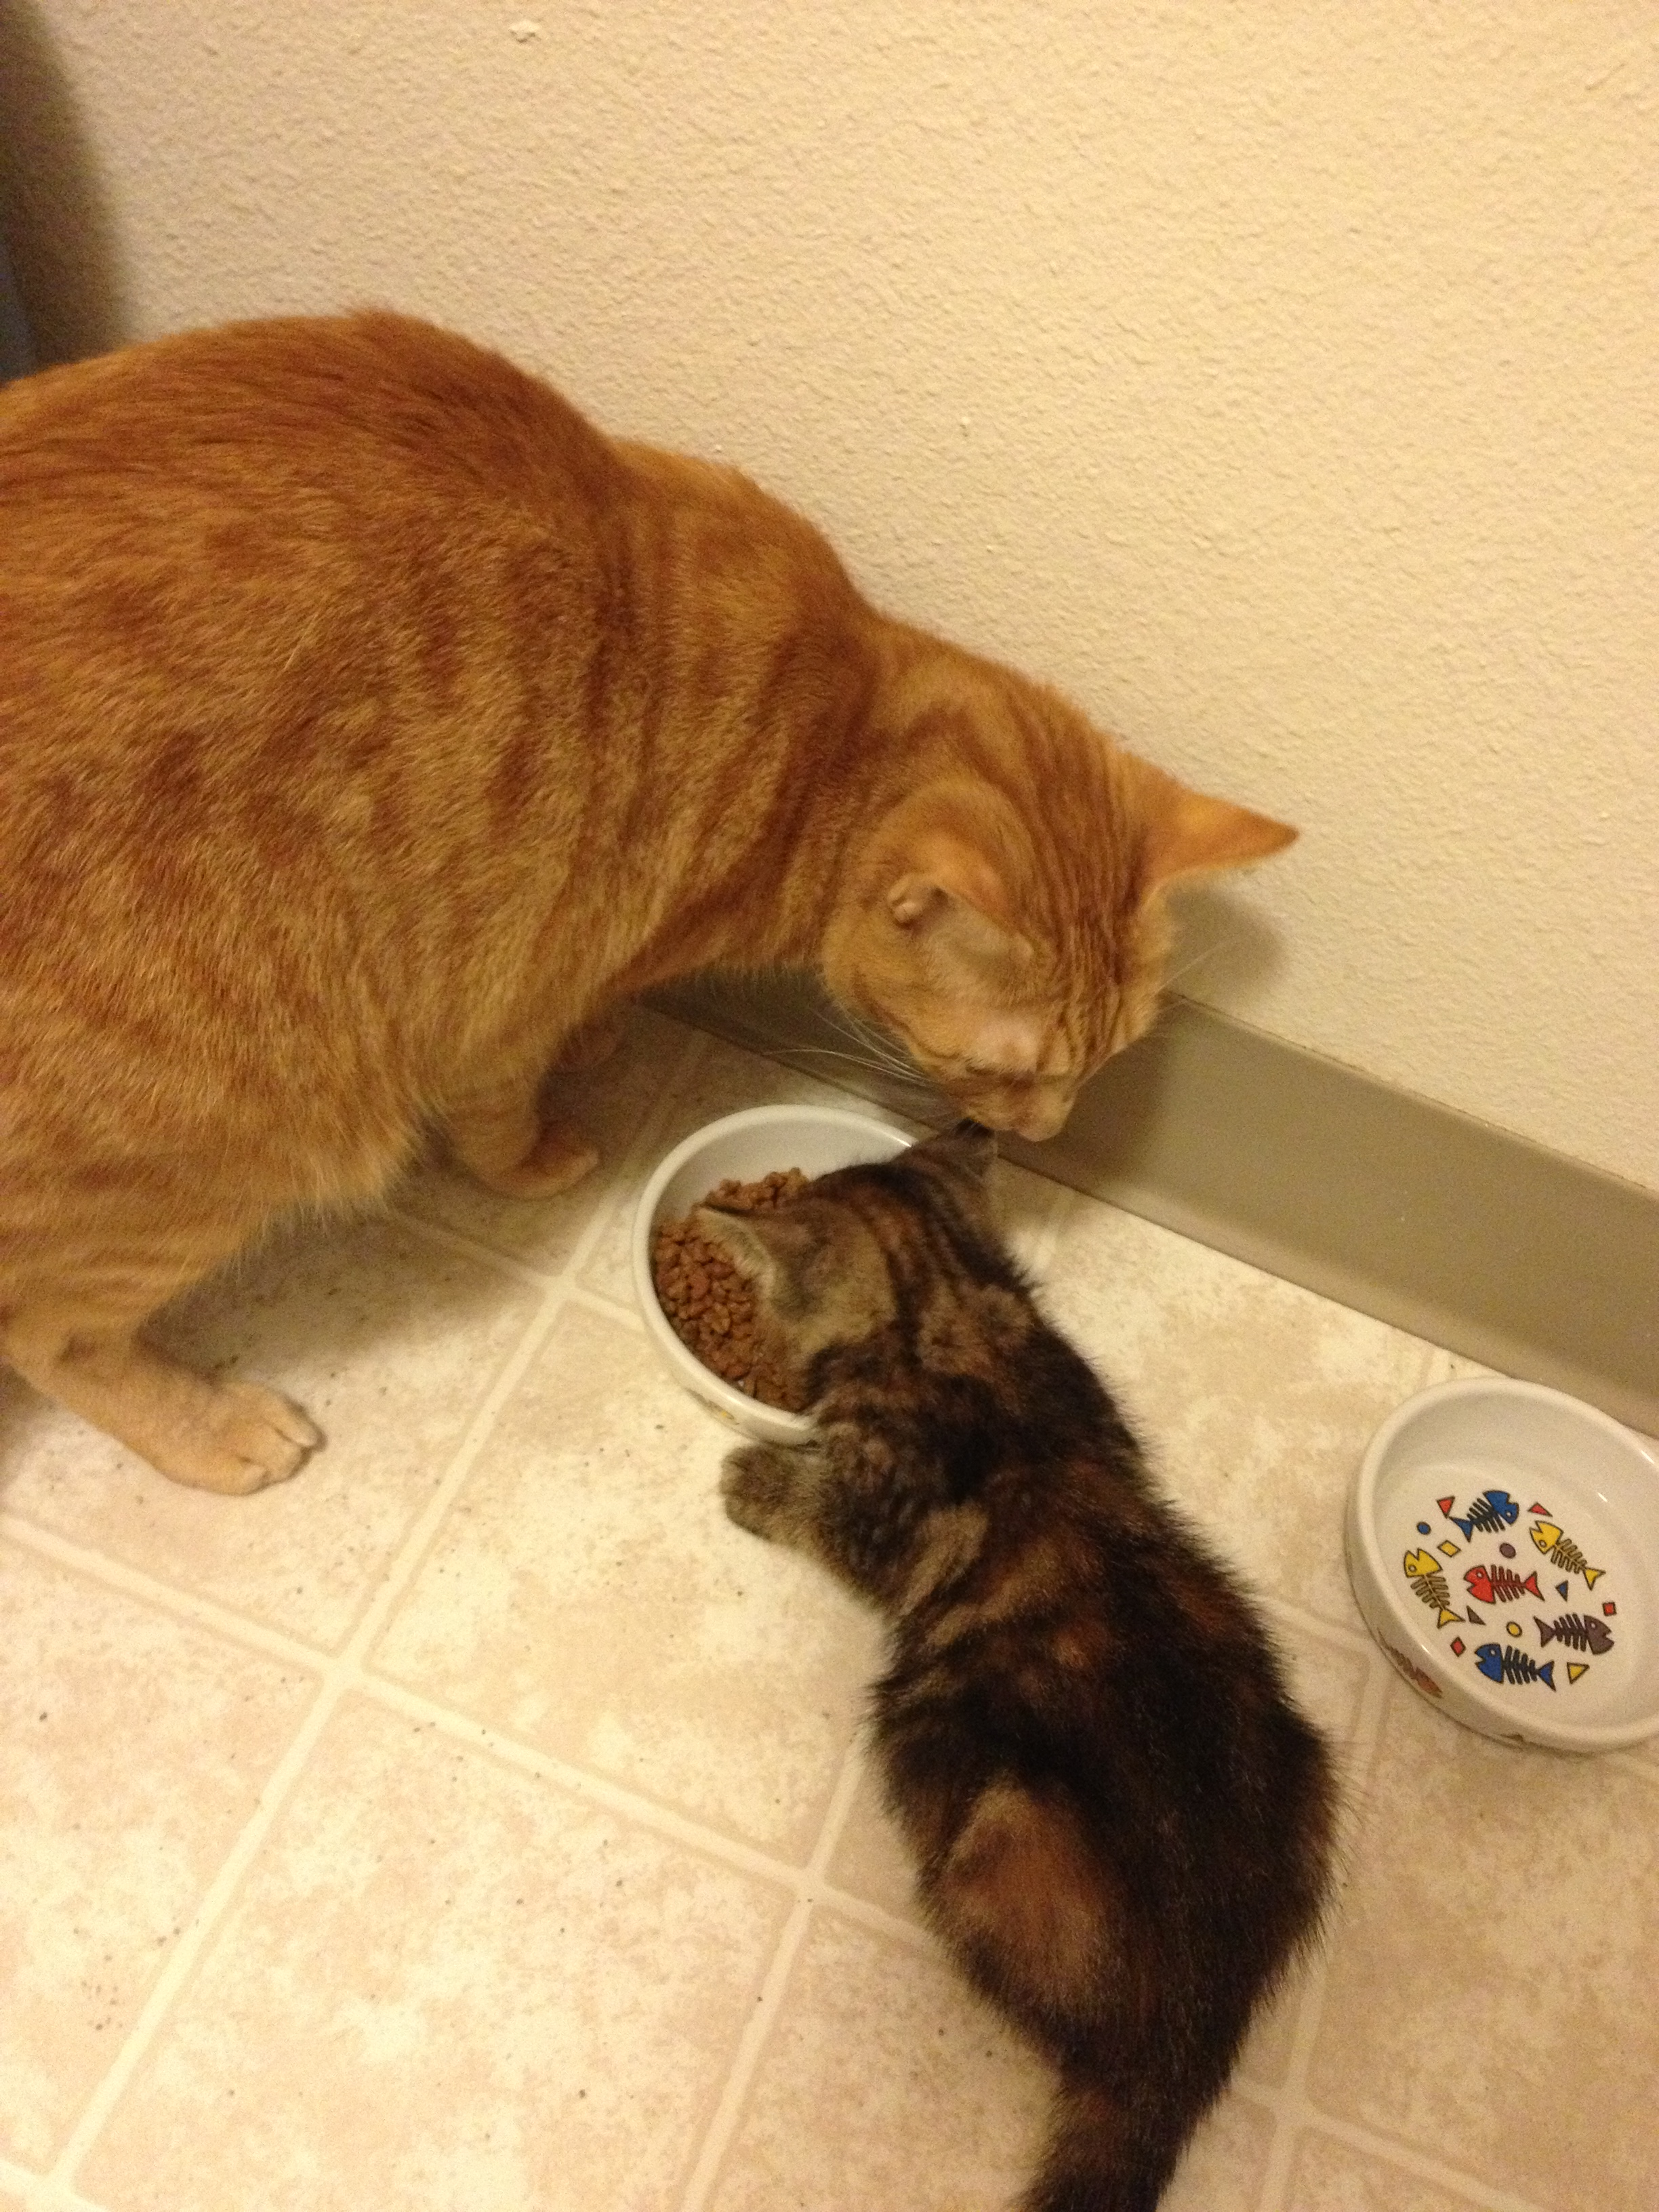
\includegraphics[width=2.5in,keepaspectratio=true]{./IMG_0886.JPG}
 % IMG_0929.JPG: 0x0 pixel, 0dpi, 0.00x0.00 cm, bb=
 \label{fig: Victor}
\end{figure}

\end{document}
